\part{Pruebas del software}
%DONE
\section{Conceptos} %25/5/17 - 3:37AM - Las fuerzas del RABENSO intentan capturarme, pero yo resistiré. Debo finalizar LA MISIÓN. "POR CORBA", gritó un transeunte mientras el escriba Almuiña seguía con ENSO. "POR JADE", respondió Almuiña. Deja las deficiniciones como  venían en las traspas. Cuernos.

\paragraph{Verificación} Proceso de evaluación de un sistema o de uno de sus componentes para determinar si los productos de una fase dada satisfacen las condiciones impuestas al principio de dicha fase (IEEE). \textit{¿Son todas las fases \textbf{coherentes} entre sí y correctas?¿Estamos \textbf{construyendo correctamente el producto}?}

\paragraph{Validación} Proceso de evaluación del sistema o de uno de sus componentes durante o al final del desarrollo para determinar si satisface los requisitos especificados (IEEE). \textit{¿Cumple el sistema con los requisitos \textbf{del cliente}?¿Estamos construyendo \textbf{el producto correcto}?}


\paragraph{Pruebas} Actividad en la que un sistema o uno de sus componentes se ejecuta en circunstancias previamente especificadas, y cuyos resultados son observados, registrados y evaluados comprobando algún aspecto.
% era para dejarlo 100% rabo
\paragraph{Caso de prueba} Conjunto de entradas, condiciones de ejecución y resultados esperados desarrollados para un objetivo particular.\\\textit{Ejemplo: ejercitar un camino concreto de un programa o verificar el cumplimiento de un determinado requisito.} % OK entonces. Vete al 100% RABO

% Esto está puesto así en las traspas? Coincide con lo que saca el intellij?
% De dónde estás sacando que genera un fallo? T
 % de las trasparrabas. pues entonces bien.
 %
 
\paragraph{Fallo} Incapacidad de un sistema o de alguno de sus componentes para realizar las funciones requeridas dentro de los requisitos de rendimiento especificados.
 
\paragraph{Defecto} Incorrección en el software que \textbf{genera un fallo}\\
\textit{Ejemplo: un proceso, una definición de datos o un paso de procesamiento incorrectos en un programa.}
% Palabra de RABO
% todo esto del rabo, 
\paragraph{Error}
\begin{itemize}
    \item Diferencia entre un valor calculado, observado o medido y el valor verdadero, especificado o teóricamente correcto.
    \item Resultado incorrecto.
    \item Defecto.
    \item Acción humana que conduce a un resultado incorrecto.
\end{itemize}

\begin{figure}[H]
  \centering
  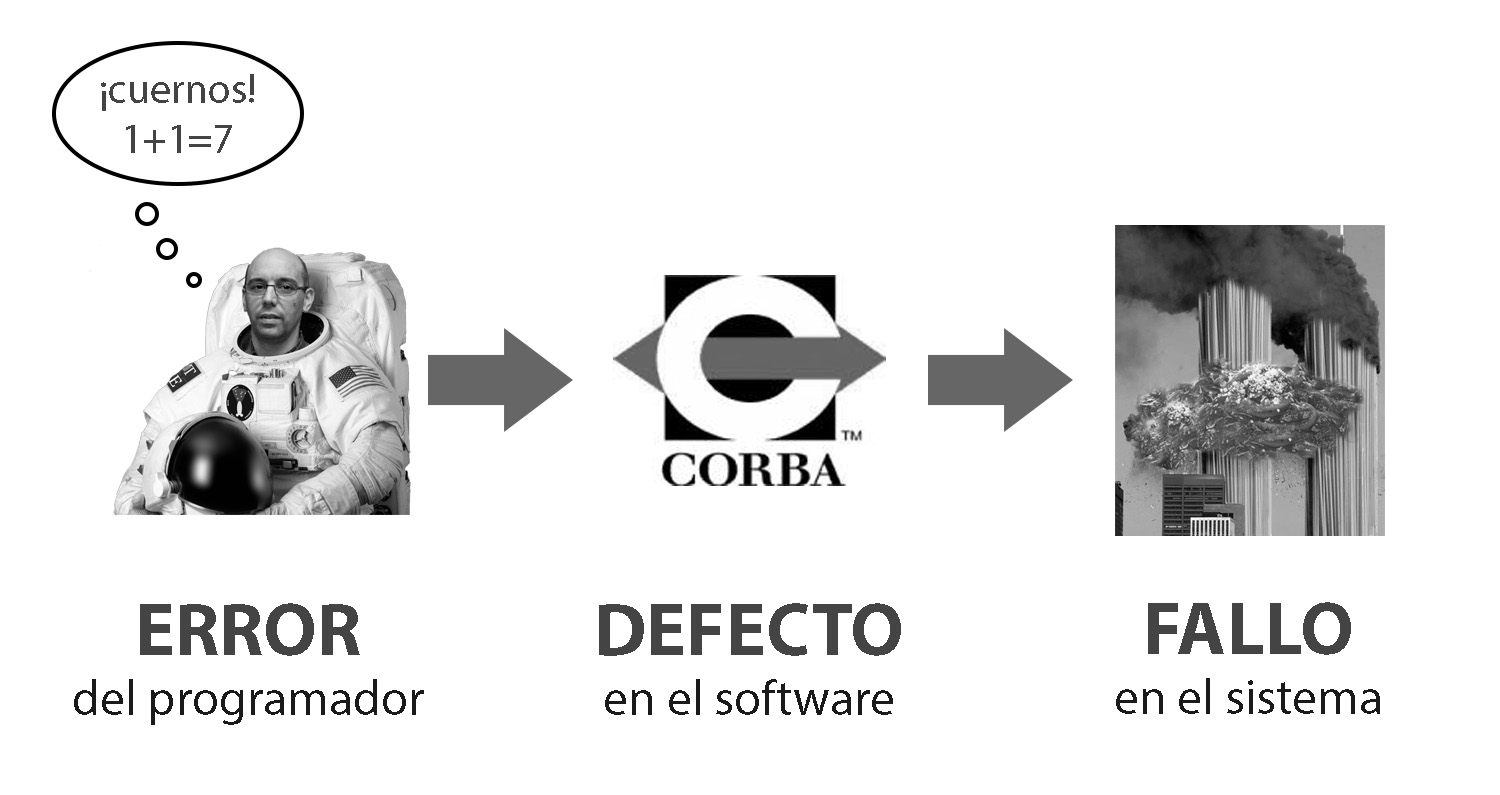
\includegraphics[width=0.8\linewidth]{Resources/cuernos}
  \caption{Recuerda: error, defecto y fallo no son lo mismo.}
  \label{fig:cuernos}
\end{figure}


\section{Filosofía de las pruebas del software}
La prueba exhaustiva del software es impracticable: \textbf{no} se pueden probar todas las posibilidades incluso en programas pequeños y sencillos. \textbf{El objetivo de las pruebas es la detección de defectos en el software en la menor cantidad de tiempo y con el menor consumo de recursos posible}.\\\\
\textbf{Descubrir un defecto constituye el éxito de la prueba}, al permitir la rectificación en el software, lo que conlleva una \textbf{mejora de la calidad}. Los defectos no siempre son el resultado de una negligencia, ya que en su aparición influyen diversos factores.

\subsection{Recomendaciones}

\begin{enumerate}
    \item \textbf{A todas las pruebas se les debería poder hacer un seguimiento hasta los requisitos del cliente}.
    \item \textbf{Las pruebas deberían planificarse mucho antes de que empiecen}: La planificación de pruebas puede comenzar tan pronto esté completo el modelo de requisitos. La definición detallada de los casos de prueba puede empezar tan pronto como el modelo de diseño se ha consolidado.
    \item \textbf{El 80\% de los errores surgen al hacer el seguimiento del 20\% de los módulos del Software (\textit{Principio de Pareto})}.
    \item \textbf{Las pruebas tendrían que hacerse de lo pequeño hacia lo grande}.
    \item \textbf{NO son posibles pruebas exhaustivas}. Sin embargo, es posible cubrir adecuadamente la lógica del programa y asegurarse de que se han aplicado todas las condiciones en el diseño a nivel de componente.
    \item \textbf{Las pruebas deberían ser realizadas por un equipo independiente del de desarrollo}: Lo ideal sería que probase el software el peor enemigo de quien lo construyó.
    \item \textbf{Cada caso de prueba debe definir el resultado de salida esperado} y compararlo con el realmente obtenido.
    \item \textbf{Se debe inspeccionar a conciencia el resultado de cada prueba} para así poder descubrir posibles síntomas de defectos.
    \item \textbf{Al generar casos de prueba se deben incluir tanto datos de entrada válidos y esperados como no válidos e inesperados}.
    \item \textbf{Las pruebas deben centrarse en probar si el software}:
    \begin{itemize}
        \item \textbf{No hace lo que debe hacer}.
        \item \textbf{Hace lo que no debe hacer}.
    \end{itemize}
    \item \textbf{Se deben evitar los casos desechables}: No documentados o diseñados sin cuidado.
    \item \textbf{No deben hacerse casos de prueba suponiendo que no hay defectos en los programas}.
    \item \textbf{Las pruebas son una tarea tanto o más creativa que el desarrollo de software}.
\end{enumerate}




% Esto no es rabo canónico
% \section{El proceso de prueba}

% \begin{enumerate}
%     \item \textbf{Generación de un plan} de pruebas. En base a la documentación sobre el proyecto y sobre el software a probar.
%     \item \textbf{Diseño} de pruebas específicas. A partir del plan.
%     \item \textbf{Ejecución} de las pruebas sobre el software.
%     \item \textbf{Evaluación} de los datos de salida. A partir de ella se pueden realizar 2 actividades:
%     \begin{itemize}
%         \item \textbf{Depuración}: Puede corregir o no los defectos; si no consigue localizarlos, puede ser necesario realizar pruebas adicionales para obtener más información. Si se corrige un defecto, se debe volver a probar el software.
%         \item \textbf{Análisis de errores}: Puede servir para realizar predicciones de la fiabilidad del software y para detectar las causas más habituales de error.
%     \end{itemize}
% \end{enumerate}

\section{Jerarquía de de la documentación de diseño de pruebas}
%Diapositiva 9 p(ongo iimamgaenge)si

De acuerdo con el \textbf{estándar IEEE 829} Se generarán la siguiente documentación:
\begin{enumerate}
    \item \textbf{Plan de pruebas}: Establece las líneas generales del plan, especificando qué elementos y funcionalidades se van a probar, personal responsable, metodologías seguidas\ldots 
    % Level Test Plan (LTP): For each LTP the scope, approach, resources, and schedule of the testing activities for its specified level of testing need to be described. The items being tested, the features to be tested, the testing tasks to be performed, the personnel responsible for each task, and the associated risk(s) need to be identified.
    \item \textbf{Especificación del diseño de pruebas}: Detalla los casos de prueba y los resultados esperados así como los criterios de paso de prueba. % Level Test Design (LTD): Detailing test cases and the expected results as well as test pass criteria.

    \item \textbf{Especificación de los casos de prueba}: Definen los datos de prueba (entradas y salidas) usados en la ejecución de los casos de prueba. % Level Test Case (LTC): Specifying the test data for use in running the test cases identified in the Level Test Design.
    
    
    \item \textbf{Especificación de procedimiento de las pruebas}: Detalla cómo se ejecutará cada uno de los casos de prueba y los pasos necesarios a seguir.
    
    \item Documentos de ejecución (\textbf{para Taboada el IEEE 1008})\footnote{Rabenso divide la documentación de pruebas en dos estándares: el IEEE 829 y el 1008. De acuerdo, con el IEEE 829--2008, esto no sería necesario pues éste estándar es más completo e incluye todas las fases.}:
    \begin{itemize}
        \item \textbf{Histórico de pruebas}: provee cronológicamente detalles relevante sobre la ejecución de las pruebas informando de cuáles fueron ejecutadas, quién las ejecutó, en qué orden y si pasaron o fallaron la prueba.
        % To provide a chronological record of relevant details about the execution of tests, e.g. recording which tests cases were run, who ran them, in what order, and whether each test passed or failed.
        \item \textbf{Informe de incidentes}: informa de cualquier problema, incidente o defecto que ocurra durante la ejecución de las pruebas que requiera investigación.
    \end{itemize}
    \item \textbf{Informe resumen de pruebas}: sumario de los resultados y evaluaciones y recomendaciones basadas en éstos. Realizado tras la finalización de la ejecución de las pruebas.
        % Level Test Report (LTR): To summarize the results of the designated testing activities and to provide evaluations and recommendations based on the results after test execution has finished for the specific test level
\end{enumerate}
\begin{figure}[H]
  \centering
  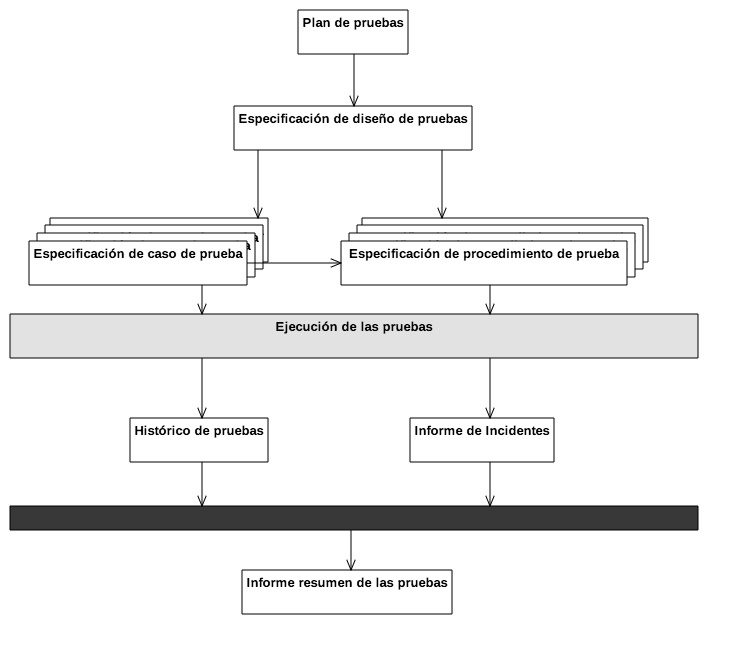
\includegraphics[width=0.6\linewidth]{Resources/IEEE829}
  \caption{El estándar IEEE 829--2008 para la realización de pruebas del software diferencia tres fases: especificación del plan de pruebas, ejecución, y elaboración de informes.}
  \label{fig:IEEE829}
\end{figure}

\section{Técnicas de diseño de casos de prueba}
Dos enfoques principales:
\begin{enumerate}
    \item \textbf{Caja negra: sólo necesitamos conocer la interfaz del elemento probado, probamos si las salidas se corresponden con la entrada. Enfoque funcional}
    \item \textbf{Caja blanca: conocemos las interioridades del sistema, probaremos que los componentes internos funcionan bien y encajan correctamente. Enfoque estructural}
\end{enumerate}
\subsection{Pruebas de caja negra (funcionales)} 

Dado que no es posible probar todo, esta sección recoge varias estrategias de creación de pruebas de caja negra que aumentan las posibilidades de descubrir errores:

\begin{enumerate}
    \item \textbf{Clases de equivalencia}: Identificamos los rangos en las restricciones de entrada o los tipos de entrada que producen un tipo de salida. Debemos \textbf{probar un valor dentro de cada rango o tipo}.
    \item \textbf{\textbf{A}nálisis de \textbf{V}alores \textbf{L}ímite (\textbf{AVL})}: Consiste en probar los errores que están en los límites de las clases de equivalencia.
    \item \textbf{Conjetura de errores}: Se prueban errores que los programadores cometen con frecuencia, bien partiendo de una lista de errores frecuentes o de la intuición del creador de la prueba.
    \item \textbf{Pruebas aleatorias}: Generamos permutaciones aleatorias de los valores de entrada y comprobamos si la salida es correcta.
\end{enumerate}

% no sale en las traspas y no me suena de clase
% \subsubsection{Métodos basados en grafos}

% La prueba del software empieza creando un grafo (colección de nodos que representan objetos, enlaces que representan relaciones entre objetos, pesos de nodos que describen las propiedades de un nodo, y pesos de enlaces que describen las características de un enlace).
% \\\\
% \uline{Métodos de prueba de comportamiento que pueden hacer uso de grafos}:
% \begin{enumerate}
%     \item \textbf{Modelado del flujo de transacción}: Los nodos representan los pasos de alguna transacción y los enlaces representan conexiones lógicas entre los pasos.
%     \item \textbf{Modelado de estado finito}: Los nodos son estados del software observables por el usuario y los enlaces son las transiciones que ocurren para moverse de un estado a otro.
%     \item \textbf{Modelado del flujo de datos}: Los nodos son objetos de datos y los enlaces son las transformaciones que ocurren para convertir un objeto de datos en otro.
% \end{enumerate}
% Cada relación en el grafo es estudiada separadamente, de manera que se puedan obtener casos de prueba. Se estudia la transitividad de relaciones secuenciales para determinar cómo se propaga el impacto de las relaciones a través de los objetos definidos en el grafo. La simetría de una relación también es importante para el diseño de casos de prueba; si un enlace es bidireccional, debería probarse esta característica. Todos los nodos del grafo deberían ser reflexivos, es decir, tener una relación que los devuelva a ellos mismos.




\subsection{Pruebas de caja blanca (estructurales)} 
El diseño de casos tiene que basarse en la \textbf{elección de caminos importantes que ofrezcan una seguridad aceptable de descubrir un defecto}, y para ello se utilizan los criterios de cobertura lógica. No requieren el uso de representaciones gráficas, pero se suelen utilizar grafos de flujo.

\begin{figure}[H]
  \centering
  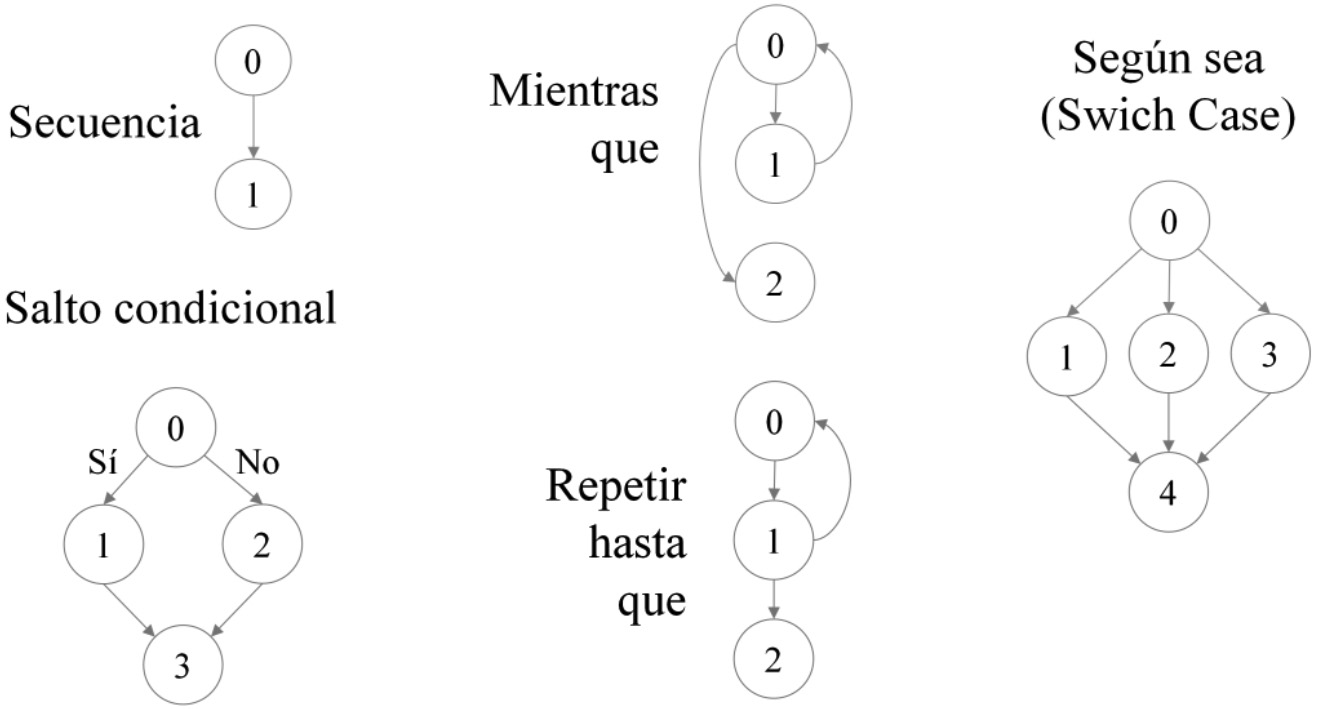
\includegraphics[width=0.6\linewidth]{Resources/ejemplosBasicosGrafos}
  \caption{Grafos básicos.}
  \label{fig:ejemplobasicografos}
\end{figure}

\subsubsection{Criterios de cobertura lógica}

\begin{enumerate}
    \item \textbf{Cobertura de sentencias}: Cada sentencia o instrucción del programa se ejecuta al menos una vez.
    
    \item \textbf{Cobertura de decisiones}: Cada decisión tiene, al menos una vez, un resultado verdadero y uno falso. En general, la cobertura de decisiones asegura la cobertura de sentencia.
    
    \item \textbf{Cobertura de condiciones}: Cada condición de cada decisión adopta, al menos una vez, un resultado verdadero y otro falso. No garantiza la cobertura de decisiones.
    
    \item \textbf{Criterio de decisión/condición}: Exigir el criterio de cobertura de condiciones obligando a que se cumpla también el criterio de decisiones.
    
    \item \textbf{Criterio de condición múltiple}: Descompone cada decisión múltiple en una secuencia de decisiones unicondicionales\footnote{una decisión es un conjunto de condiciones, por ejemplo en 
    \texttt{a != null \&\& a.leng > 3} es una decisión que se descompone en las condiciones \texttt{a != null} y \texttt{a.leng > 3}} y luego se exige que cada combinación posible de resultados de cada condición se ejecute al menos una vez. %WTF condiciones unicondicionales, eso hay que revisarlo…
    
    \item \textbf{Cobertura de caminos}: Cada uno de los posibles caminos del grafo de caminos  se ejecuta al menos una vez. Según las veces que recorramos el bucle tenemos diferentes tipos:
    \begin{itemize}
        \item Sin entrar en su interior.
        \item Ejecutándolo una vez.
        \item Ejecutándolo dos veces.
        \item Ejecutándolo n veces.
    \end{itemize}
\end{enumerate}



\subsubsection{Prueba de bucles}
La prueba de bucles es la \textbf{técnica de prueba de caja blanca que se centra exclusivamente en la validez de las construcciones de bucles}. Se pueden definir 4 clases de bucles:
\begin{enumerate}
    \item \textbf{Bucles simples}: Se les debe aplicar el siguiente conjunto de pruebas:
    \begin{itemize}
        \item Pasarlo por alto.
        \item Pasar una vez por el bucle.
        \item Pasar 2 veces por el bucle.
        \item Hacer $m$ pasos con $m < n$ tal que $n$ es el mayor número de pasos permitidos por el bucle.
        \item Hacer $n-1$ y $n+1$ pasos
    \end{itemize}
    \item \textbf{Bucles anidados}:
    \begin{itemize}
        \item Comenzar por el bucle más interior con los otros en sus valores mínimos.
        \item Llevar a cabo la prueba de bucle simple al más interior.
        \item Progresar hacia fuera, manteniendo el resto de bucles externos en sus valores mínimos y los demás bucles anidados en sus valores típicos.
        \item Continuar hasta probar todos los bucles.
    \end{itemize}
    \item \textbf{Bucles concatenados}: Se pueden probar mediante el enfoque para bucles simples siempre que cada bucle sea independiente del resto. Si son dependientes se usa la técnica para bucles anidados.
    \item \textbf{Bucles no estructurados}: Se deben rediseñar para que se ajusten a las construcciones de la programación estructurada.
\end{enumerate}



\subsubsection{Utilización de la complejidad ciclomática de McCabe}
La \textbf{métrica de McCabe es un indicador del número de caminos independientes que existen en un grafo}.\\
El propio McCabe definió como un buen criterio de prueba la consecución de la ejecución de un conjunto de caminos independientes, lo que implica probar un número de caminos igual al de la métrica. La métrica de McCabe \textbf{asegura la cobertura de sentencia y sería equivalente a la cobertura de decisiones}.
\\\\
\textbf{Un camino es independiente de otros si incorpora un arco que los demás no incluyen}. La métrica de McCabe coincide con el número máximo de caminos independientes que puede haber en un grafo. \uline{Formas de calcular la complejidad ciclomática de McCabe}:
\begin{enumerate}
    \item $V (G) = a-n+2$, siendo $a$ el número de arcos y $n$, el de nodos.
    \item $V (G) = r$, siendo $r$ el número de regiones cerradas del grafo. Si el programa tiene un nodo de inicio y otro de final, la región externa se suma como región cerrada.
    \item $V (G) = c+1$, siendo $c$ el número de nodos de condición.
\end{enumerate}

Para ayudar a la elección de los caminos de prueba, McCabe propone el \textbf{método del camino básico, consistente en realizar variaciones sobre la elección de un primer camino de prueba típico}. A partir de estos caminos, se analiza el código para conocer los datos de entrada necesarios, y se consulta la especificación para conocer la salida teóricamente correcta.\\\\
\textbf{Puede suceder que las condiciones necesarias para que la ejecución pase por un determinado camino no se puedan satisfacer de ninguna manera (camino imposible}), en cuyo caso deberemos sustituir ese camino por otro posible que permita satisfacer igualmente el criterio de prueba de McCabe.
\\\\
$V (G)$ marca un límite mínimo de número de casos de prueba para un programa. Si $V (G)$ es mayor que 10, la probabilidad de encontrar defectos aumenta, salvo que sea debido a sentencias \textit{switch case} o similares. En estos casos se debe replantear el diseño modular obtenido.



\section{Enfoque práctico recomendado para el diseño de casos}

\begin{enumerate}
    \item \textbf{Si la especificación contiene combinaciones de condiciones de entrada, comenzar formando sus grafos causa--efecto}.
    \item \textbf{Usar el análisis de valores límite (AVL) para añadir casos de prueba}: Elegir límites para dar valores a las causas en los casos generados, asumiendo que cada caso es una clase de equivalencia.
    \item \textbf{Identificar las clases válidas y no válidas de equivalencia para la entrada y la salida y añadir los casos no incluidos anteriormente}.
    \item \textbf{Utilizar conjetura de errores para añadir nuevos casos referidos a valores especiales}.
    \item \textbf{Ejecutar los casos generados hasta el momento y analizar la cobertura obtenida}.
    \item \textbf{Examinar la lógica del programa para añadir los casos precisos para cubrir el criterio de cobertura elegido} si no ha sido satisfecho en el punto anterior.
\end{enumerate}

Esto es \textbf{aplicable tanto a pruebas de caja blanca como de caja negra} ya que:
\begin{itemize}
    \item Los errores lógicos y las suposiciones incorrectas son inversamente proporcionales a la probabilidad de que se ejecute un camino del programa.
    \item Se suele creer que un determinado camino tiene pocas probabilidades de ejecutarse cuando se ejecuta regularmente.
    \item Los errores tipográficos son aleatorios.
    \item La probabilidad e importancia de un trozo de código se suele calcular de modo subjetivo.
    \item Una prueba exhaustiva de caja blanca no asegura la detección de los defectos de su diseño.
\end{itemize}



\subsection{Depuración}
La depuración es el \textbf{proceso de localizar, analizar y corregir los defectos que se sospecha que contiene el software}. Suele ser la consecuencia de una prueba con éxito. Tras corregir el defecto, se efectuarán nuevas pruebas que comprueben si se ha eliminado dicho problema.

\subsection{Análisis de errores a análisis causal}
El análisis causal \textbf{proporciona información sobre la naturaleza de los defectos para que así el personal pueda prevenirlos en el futuro}. Se recoge la siguiente información:
\begin{itemize}
    \item Cuándo se cometió.
    \item Quién lo cometió.
    \item Qué se hizo mal.
    \item Cómo se podría haber prevenido.
    \item Por qué no se detectó antes.
    \item Cómo se podría haber detectado antes.
    \item Cómo se encontró el error.
\end{itemize}

No debe usarse para evaluar al personal.

\section{Estrategia de aplicación de las pruebas}
%gráfico traspa 87
\begin{enumerate} % 
    \item \textbf{Prueba de unidad}: Se centra en ejercitar la lógica del módulo y los distintos aspectos de la especificación de las funciones que debe realizar el módulo.
    \item \textbf{Prueba de integración}: Debe tener en cuenta los mecanismos de agrupación de módulos fijados en la estructura del programa, así como las interfaces entre componentes.
    %\item \textbf{Prueba de validación}: Debe comprobar si existen desajustes entre el software y los requisitos fijados para su funcionamiento en la especificación de requisitos software (ERS). %Esta prueba no está en las trasparrabas. Por lo tanto, no existe
    \item \textbf{Prueba del sistema}: Debe comprobar el cumplimiento de los objetivos indicados para el sistema.
    \item \textbf{Prueba de aceptación}: El usuario verifica en su entorno si acepta el producto.
\end{enumerate}
\begin{figure}[H]
  \centering
  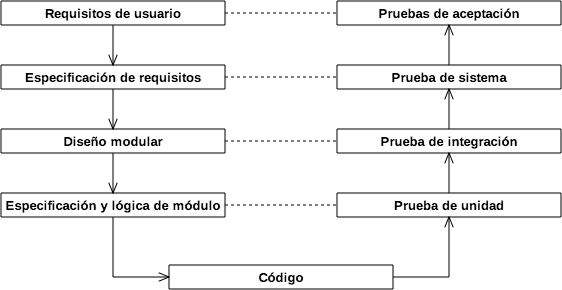
\includegraphics[width=0.7\linewidth]{Resources/enfoquePruebas}
  \caption{Las diferentes estrategias de prueba y su relación con las otras fases del construcción del software}
  \label{fig:estrategiasPruebas}
\end{figure}


\newpage
\section{Pruebas en desarrollos orientados a objetos}
\subsection{Desde el punto de vista de diseño de casos de pruebas}
\begin{itemize}
    \item \textbf{Las técnicas de caja negra}: Totalmente válidas.
    \begin{itemize}
        \item Análisis de valores límite, tratamiento de combinaciones de entrada y conjetura de errores.
        \item Debemos diseñar las pruebas basándonos en datos y eventos de los escenarios de los casos de uso y en flujos alternativos, tratamientos de error y excepciones.
    \end{itemize}
    \item \textbf{Las técnicas de caja blanca}: Disminuyen sus posibilidades de aplicación. Quedan confinadas a las instrucciones de cada método de cada clase.
\end{itemize}

\subsection{Desde el punto de vista del nivel}
Los cambios más radicales aparecen en las pruebas de integración, cuando nos fijamos en la interacción entre objetos de distintas clases. El enfoque habitual consiste en ir probando hilos de clases que colaboran para una función o servicio del sistema.

\subsection{Cuestiones a tener en cuenta}
Ciertas cuestiones a tener en cuenta a la hora de probar software orientado a objetos son:
\begin{itemize}
\item \textbf{Herencia}: probar un método de la clase padre no garantiza su funcionamiento en clases hijas.
\item \textbf{Polimorfismo}: un único método puede tener implementaciones diferentes en función de la clase en la que se use.
    \item Es conveniente recordar que la propia programación o diseño orientado a objetos hace menos probables ciertos tipos de error, más probables otros, y provoca la aparición de nuevos tipos de defectos. %Pues OC, mejor redactado.
\end{itemize}

\newpage
\section{Ejemplo práctico de cálculo de la complejidad ciclomática de un método}
Dado el método  \texttt{public String porcentajeVentasMes();} tal que: 
\begin{verbatim}
public String porcentajeVentasMes() {
	    [...]
	//recopilamos precios por dia
    for(int i = 0 ; i < ventas.size() ; i++ ){
        Venta v=ventas.get(i);
        Calendar cal = Calendar.getInstance();
        targetCalendar.setTime(cFecha.toDate(v.getFecha()));
        precios[cal.get(Calendar.DAY_OF_MONTH)]+=v.getPrecioUnidad();
        total+=v.getPrecioUnidad();
    }

    //calcula los porcentajes
    for(int i = 0 ; i < columnas; i++ ){
        if(precios[i]>0){
        	porcentajeVentas+="Día "+(i+1)+": "+
        	+ BigDecimal.valueOf(precios[i]/total*100)
        		        .setScale(2, RoundingMode.HALF_UP)
        		        .doubleValue()+"%\n";
        }
        return porcentajeVentas;
    }
}   
\end{verbatim}

\begin{figure}[H]
  \centering
  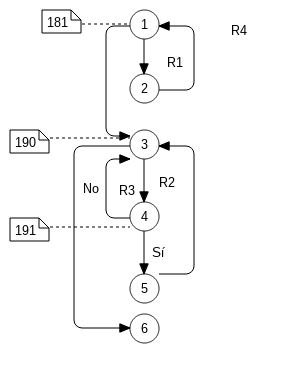
\includegraphics[width=0.4\linewidth]{Resources/porcentajeVentasMes}
  \caption{Grafo de flujo del método.}
  \label{fig:joder}
\end{figure}
\newpage
\paragraph{Caminos básicos obtenidos}
    \begin{enumerate}
        \item 1-3-6
        \item 1-\underline{2}-1-3-6
        \item 1-3-\underline{4}-3-6
        \item 1-2-3-4-\underline{5}-3-6
    \end{enumerate}

\paragraph{Caminos independientes:} 3
    \begin{enumerate}
        \item 1-(3-4)\textsuperscript{x31}-3-6
            \begin{itemize}
                \item No puede existir en el sistema ninguna venta realizada en el mes actual.
                \item La variable \texttt{columnas} sólo podrá poseer los valores 28, 29, 30 ó 31, dependiendo del mes en el que es ejecutada la función. Es por esto que no se puede llevar a cabo ningún camino que contenga 1-3-6.
            \end{itemize}
        \item 1-2-(3-4)\textsuperscript{x31}-3-6
            \begin{itemize}
                \item Para seguir este camino independiente, deberá existir  una venta realizada en el mes actual, o más si se desea repetir más veces el segmento 1-2.
                \item Ningún artículo podrá tener un precio superior a 0 para poder seguir este camino estrictamente.
            \end{itemize}
        \item 1-(3-4)\textsuperscript{x31}-3-6
            \begin{itemize}
                \item Equivalente al camino 1.
            \end{itemize}
        \item 1-2-(3-(4\textbar{}\textbar{}(4-5)))\textsuperscript{x31}-3-6
            \begin{itemize}
                \item Para seguir este camino independiente, deberá existir  una venta realizada en el mes actual con un precio por unidad superior a 0 o más si se desea repetir más veces el segmento 3-4-5.
            \end{itemize}
    \end{enumerate}
